\documentclass{beamer}
\usepackage{amsmath,amssymb,latexsym,array,fancyheadings,mathdots}
\usepackage{algorithm,algorithmic}
\usepackage{hyperref}
\usepackage{color}
\usepackage{tabularx}
\usepackage[all]{xy}
\usepackage{qtree}
\usepackage{gitinfo2}

%% RCS
%\usepackage{rcs}

%% Colors
\definecolor{darkgreen}{rgb}{0,.4,0}
\definecolor{darkred}{rgb}{.5,0,0}
\definecolor{darkmagenta}{rgb}{.5,0,.5}
\definecolor{orange}{rgb}{1,.5,0}
\definecolor{lightblue}{rgb}{0.122,0.016,0.855}
\definecolor{darkocre}{rgb}{0.471,0.298,0.008}

\usetheme{default}

%% New Theorems
\newtheorem{thm}{Theorem}
\newtheorem{exm}[thm]{Example}
\newtheorem{cor}[thm]{Corollary}
\newtheorem{propo}[thm]{Proposition}
\newtheorem{lem}[thm]{Lemma}
\newtheorem{clm}[thm]{Claim}
\newtheorem{exr}[thm]{Exercise}
\newtheorem{dfn}[thm]{Definition}

%% New commands
\newcommand{\classfont}{\mathsf}
\newcommand{\ATM}{\classfont{A}_{\mathrm{TM}}}
\newcommand{\MTF}{\mathrm{MTF}}
\newcommand{\OPT}{\mathrm{OPT}}
\newcommand{\ALG}{\mathrm{ALG}}
\newcommand{\ALGNAIVE}{\mathrm{ALG}_{\text{na{\"\i}ve}}}
\newcommand{\LRU}{\mathrm{LRU}}
\newcommand{\FIFO}{\mathrm{FIFO}}
\newcommand{\FWF}{\mathrm{FWF}}
\newcommand{\LFD}{\mathrm{LFD}}
\newcommand{\true}{\mathsf{T}}
\newcommand{\false}{\mathsf{F}}
\newcommand{\also}{\wedge}
\newcommand{\lra}{\leftrightarrow}
\newcommand{\tc}{\textcolor}
\newcommand{\df}[1]{\textcolor{red}{\em #1}}
\newcommand{\highlight}[1]{\textcolor{orange}{\em #1}}
\newcommand{\hl}[1]{\textcolor{blue}{\em #1}}
\newcommand{\amp}{\texttt{\&}}
\newcommand{\hsh}{\texttt{\#}}
\newcommand{\ra}{\rightarrow}
\newcommand{\longra}{\longrightarrow}
\newcommand{\Ra}{\Rightarrow}
\newcommand{\rab}{{\rightarrow_\beta}}
\newcommand{\srab}{{\rightarrow^*_\beta}}
\newcommand{\aeq}{{=_\alpha}}
\newcommand{\order}{\mathrm{order}}
\newcommand{\rem}{\mathrm{rem}}
\newcommand{\IP}{\mathbf{IP}}
\newcommand{\PSPACE}{\mathbf{PSPACE}}
\newcommand{\thevalue}{\text{value}}
\newcommand{\pol}[1]{\mathbf{#1}}
\newcommand{\enc}{\text{Enc}}
\newcommand{\xor}{\oplus}
\newcommand{\zo}{\{0,1\}}
\newcommand{\SOPT}{S_{\mathrm{opt}}}
\newcommand{\la}{\leftarrow}
\newcommand{\myurl}[1]{\textcolor{darkgreen}{\url{#1}}}
\newcommand{\myhref}[2]{\textcolor{darkgreen}{\href{#1}{#2}}}
\newcommand{\qaccept}{q_{\mathrm{accept}}}
\newcommand{\qreject}{q_{\mathrm{reject}}}
\newcommand{\opt}{\text{\sc Opt}}
\newcommand{\tr}{\mathrm{tr}}
\newcommand{\csanky}{p^{\textsc{csanky}}}
\newcommand{\berk}{p^{\textsc{berk}}}

%% Algorithms package customization
\renewcommand{\algorithmicrequire}{\textbf{Pre-condition:}} 
\renewcommand{\algorithmicensure}{\textbf{Post-condition:}} 
\algsetup{indent=3em}

\input{prooftree}

%% including/excluding pauses
\newcommand{\ifpause}{\iftrue} % for including pauses
%\newcommand{\ifpause}{\iffalse} % for excluding pauses

%% 2nd or 3rd edition
\newif\ifthird
\thirdtrue
%\thirdfalse

%disables usefoottemplate
\setbeamertemplate{navigation symbols}{}
%\setbeamertemplate{footline}% 
%{\strut\quad\tiny 
%\begin{minipage}{3cm}
%Cryptography - Michael Soltys
%\today\ {\tt v\RCSRevision}
%\end{minipage}\hfill
%\insertsection\
%- \insertframenumber/\inserttotalframenumber\quad\strut}

\newcommand{\mytitle}{Computational Foundations: Turing Machines}
\newcommand{\mychpnr}{9}
%% Title page contents
\title{Intro to Analysis of Algorithms \\ \mytitle \\  Chapter \mychpnr}
\author{Michael Soltys}
\date{\textcolor{darkgreen}{\tiny\tt 
[ {\bf Git} Date:\gitAuthorDate\ 
Hash:\gitAbbrevHash\ 
Ed:\ifthird
3rd
\else
2nd
\fi]}}
\institute{CSU Channel Islands}

\setbeamertemplate{footline}{
  \colorbox{white}{\color{black}\tt
     \begin{tabularx}{0.97\textwidth}{XXX}
          IAA Chp \mychpnr\ - Michael Soltys \copyright & 
          \hfill\today\ (\gitAbbrevHash; \ifthird ed3\else ed2\fi)
					\hfill\phantom{.} & 
          \hfill\insertsection\ - \insertframenumber/\inserttotalframenumber \\
      \end{tabularx}}}

\begin{document}

\mode<presentation>
{
}

\parskip 8pt

\section{Introduction}

\begin{frame}
\titlepage
\end{frame}


\begin{frame}
\begin{center}
\addtocounter{part}{1}
{\bf Part \Roman{part} \\ Turing machines}
\end{center}
\end{frame}

\begin{frame}
Finite control and an infinite tape.

Initially the input is placed on the tape, the head of the tape is
reading the first symbol of the input, and the state is $q_0$.

The other squares contain blanks.

Formally, a \df{Turing machine} is a tuple 
$(Q,\Sigma,\Gamma,\delta)$

where $Q$ is a finite set of \df{states} (always
including the three special states $q_{\text{init}}$,
$q_{\text{accept}}$ and
$q_{\text{reject}}$)

$\Sigma$ is a finite \df{input alphabet} 

$\Gamma$ is a finite \df{tape
alphabet}, and it is always the case that $\Sigma\subseteq\Gamma$ (it
is convenient to have symbols on the tape which are never part of the
input),
$$
\delta:Q\times\Gamma\rightarrow
Q\times\Gamma\times\{\text{Left},\text{Right}\}
$$ 
is the \df{transition function}
\end{frame}

\begin{frame}
\begin{minipage}{5cm}
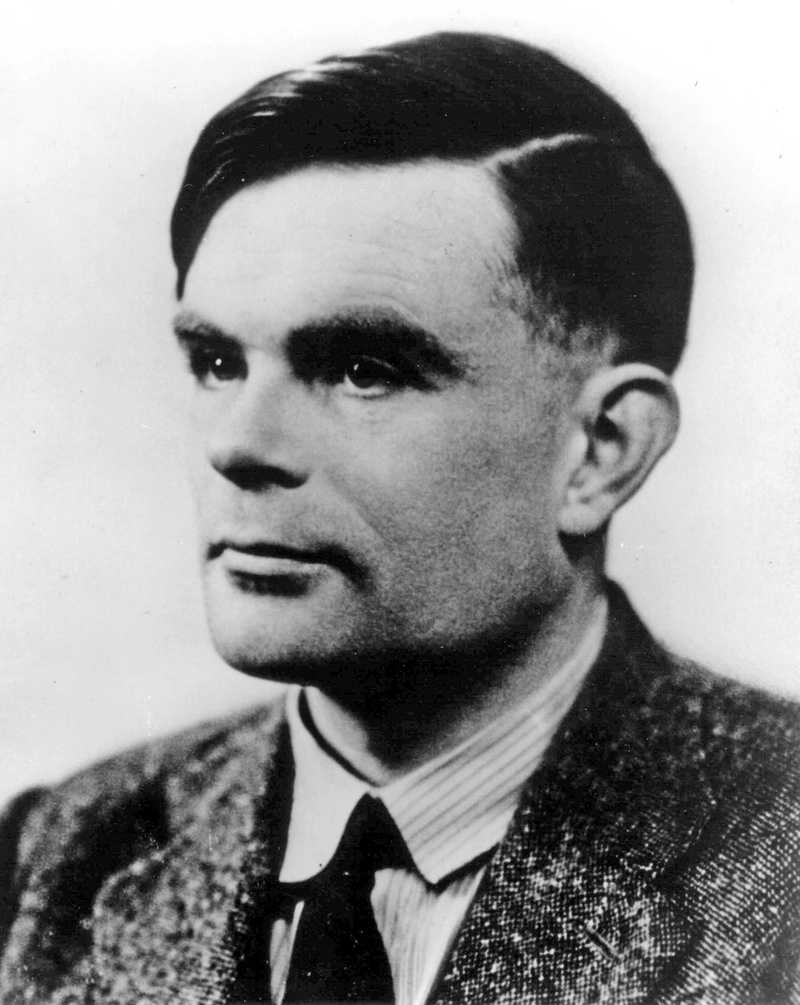
\includegraphics[width=4cm]{figures/AlanTuring.jpg}
\end{minipage}
\begin{minipage}{5cm}
\myhref{http://en.wikipedia.org/wiki/Alan_Turing}{Alan Turing} \\
\end{minipage}
\end{frame}

\begin{frame}
A \df{configuration} is a tuple $(q,w,u)$ where
$q\in Q$ is a state, and where $w,u\in\Gamma^*$, the cursor is on the
last symbol of $w$, and $u$ is the string to the right of $w$.  

A configuration $(q,w,u)$ \df{yields} 
$(q',w',u')$ in one step, denoted as
$(q,w,u)\stackrel{M}{\rightarrow}(q',w',u')$ if one step of $M$ on
$(q,w,u)$ results in $(q',w',u')$.  

Analogously, we
define $\stackrel{M^k}{\rightarrow}$, yields in $k$ steps, and
$\stackrel{M^*}{\rightarrow}$, yields in any number of steps,
including zero steps.  

The initial configuration, $C_{\text{init}}$,
is $(q_{\text{init}},\triangleright,x)$ where $q_{\text{init}}$ is the
initial state, $x$ is the input, and $\triangleright$ is the left-most
tape symbol, which is always there to indicate the left-end of the
tape.
\end{frame}

\begin{frame}
Given a string $w$ as input, we ``turn on'' the TM in the initial
configuration $C_{\text{init}}$, and the machine moves from
configuration to configuration.  

The computation ends when either the
state $q_{\text{accept}}$ is entered, in which case we say that the TM
{\em accepts} $w$, or the state $q_{\text{reject}}$ is entered, in
which case we say that the TM {\em rejects} $w$.  It is possible for
the TM to never enter $q_{\text{accept}}$ or $q_{\text{reject}}$, in
which case the computation does not halt.

Given a TM $M$ we define $L(M)$ to be the set of strings accepted by
$M$, i.e., $L(M)=\{x|\text{$M$ accepts $x$}\}$, or, put another way,
$L(M)$ is the set of precisely those strings $x$ for which
$(q_{\text{init}},\triangleright,x)$ yields an accepting
configuration.
\end{frame}

\begin{frame}
Alan Turing showed the existence of a so called \df{Universal
Turing machine} (UTM); a UTM
is capable of simulating any TM from its description.

A UTM is what we mean by a \df{computer}, capable of running
any algorithm.  The proof is not
difficult, but it requires care in defining a consistent way of
presenting TMs and inputs.

Every Computer Scientist should at some point write a UTM in their
favorite programming language $\ldots$

This exercise really means: designing your own programming language
(how you present descriptions of TMs); designing your own compiler
(how your machine interprets those ``descriptions''); etc.
\end{frame}

\begin{frame}
\df{NTM}

$N$ s.t. $L(N)=\{w\in\{0,1\}^*|\text{ last
symbol of $w$ is 1 }\}$.

\begin{minipage}{5cm}
\begin{align*}
\delta(q_0,0) &=\{(q_0,0,\rightarrow),(q,0,\rightarrow)\} \\
\delta(q_0,1) &=\{(q_0,1,\rightarrow),(r,1,\rightarrow)\} \\
\delta(r,\square) &=\{(\qaccept,\square,\rightarrow)\} \\
\delta(r,0/1) &=\{(q,0,\rightarrow)\}
\end{align*}
\end{minipage}
\begin{minipage}{4cm}
\begin{center}
\Tree [.$q_0011$ [.$0q_011$ [.$01q_01$ [.$011q_0$ $\times$ ] 
[.$011r$ $011\square \qaccept$  ] ] 
[.$01r1$ [.$010q$ $\times$ ] ] ] [.$0q11$ $\times$ ] ] 
\end{center}
\end{minipage}
\end{frame}

\begin{frame}
Different variants of TMs are equivalent (\df{robustness}):
tape infinite in only one direction, or
several tapes.

TM $=$ NTM:
$D$ maintains a sequence of config's on tape 1:
$$
\begin{array}{c|c|c|c|c}\hline
\cdots & \text{config}_1 & \text{config}_2 & \text{config}_3^* & \cdots \\\hline
\end{array}
$$
and uses a second tape for scratch work.

The marked config (*) is the current config.  $D$ copies it to the second
tape, and examines it to see if it is accepting.  If it is, it accepts.

If it is not, and $N$ has $k$ possible moves, $D$ copies the $k$ new
config's resulting from these moves at the end of tape 1, and marks the
next config as current. 

If max nr of choices of $N$ is $m$, and $N$ makes $n$ moves, $D$
examines $1+m+m^2+m^3+\cdots+m^n\approx nm^n$ many configs.
\end{frame}

\begin{frame}

{\bf Undecidability}

We can encode every Turing machine with a string over $\{0,1\}$.  For
example, if $M$ is a TM:
$$
(\{q_1,q_2\},\{0,1\},\delta,\ldots)
$$
and $\delta(q_1,1)=(q_2,0,\rightarrow)$ is one of the transitions,
then it could be encoded as:
$$
\underbrace{0}_{q_1}1
\underbrace{00}_11
\underbrace{00}_{q_2}1
\underbrace{0}_01
\underbrace{0}_\rightarrow11
\underbrace{\ldots\ldots\ldots\ldots\ldots\ldots}_{
\text{\begin{minipage}{3cm}encoding of other\\[-3mm]transitions\end{minipage}}}
$$

Not every string is going to be a valid encoding of a TM (for example
the string 1 does not encode anything in our convention).  

Let all ``bad strings'' encode a default TM $M_{\text{default}}$ which
has one state, and halts immediately, so
$L(M_{\text{default}})=\emptyset$.
\end{frame}

\begin{frame}

\begin{quote}
{\em The intuitive notion of algorithm is captured by the formal
definition of a TM.}
\end{quote}

$$
\ATM=\{\langle M,w\rangle:\text{$M$ is a TM and $M$ accepts
$w$}\},
$$
called the {\em universal language}
\end{frame}

\begin{frame}

{\bf Theorem 6.63:} $\ATM$ is undecidable.


Suppose that it is decidable, and that $H$ decides it.  Then,
$L(H)=\ATM$, and $H$ always halts (observe that $L(H)=L(U)$, but $U$,
as we already mentioned, is not guaranteed to be a decider).  Define a
new machine $D$ (here $D$ stands for ``diagonal,'' since this argument
follows Cantor's ``diagonal argument''):
$$
D(\langle M\rangle):=
\begin{cases}
\text{accept} & \text{if $H(\langle M,\langle M\rangle\rangle)=$ reject} \\
\text{reject} & \text{if $H(\langle M,\langle M\rangle\rangle)=$ accept}
\end{cases}
$$
that is, $D$ does the ``opposite.''  Then we can see that $D(\langle
D\rangle)$ accepts iff it rejects.  Contradiction; so $\ATM$ cannot be
decidable.

\end{frame}

\begin{frame}
It turns out that all nontrivial properties of RE languages are
undecidable, in the sense that the language consisting of codes of TMs
having this property is not recursive.

E.g., the language consisting of codes of TMs whose languages are
empty (i.e., $L_e$) is not recursive.

A \df{property} of RE languages is simply a subset of RE.  A property
is \df{trivial} if it is empty or if it is everything.

If $\mathcal{P}$ is a property of RE languages, the language
$L_{\mathcal{P}}$ is the set of codes for TMs $M_i$ s.t.
$L(M_i)\in\mathcal{P}$.

When we talk about the decidability of $\mathcal{P}$, we formally mean
the decidability of $L_{\mathcal{P}}$.
\end{frame}

\begin{frame}

{\bf Rice's Theorem:} Every nontrivial property of RE languages is
undecidable.

Proof: Suppose $\mathcal{P}$ is nontrivial.  Assume
$\emptyset\not\in\mathcal{P}$ (if it is, consider
$\overline{\mathcal{P}}$ which is also nontrivial).

Since $\mathcal{P}$ is nontrivial, some $L\in\mathcal{P}$,
$L\neq\emptyset$. 

Let $M_L$ be the TM accepting $L$.

For a fixed pair $(M,w)$ consider the TM $M'$: on input $x$, it first
simulates $M(w)$, and if it accepts, it simulates $M_L(x)$, and if
that accepts, $M'$ accepts.

$\therefore$ $L(M')=\emptyset\not\in\mathcal{P}$ if $M$ does not
accept $w$, and $L(M')=L\in\mathcal{P}$ if $M$ accepts $w$.

Thus, $L(M')\in\mathcal{P}\iff(M,w)\in \ATM$, $\therefore$
$\mathcal{P}$ is undecidable.
\end{frame}

\begin{frame}

{\bf Post's Correspondence Problem (PCP)}

An instance of \df{PCP} consists of two finite lists of strings over
some alphabet $\Sigma$.  The two lists must be of equal length:

$A=w_1,w_2,\ldots,w_k$ \\
$B=x_1,x_2,\ldots,x_k$

For each $i$, the pair $(w_i,x_i)$ is said to be a \df{corresponding
pair}.  We say that this instance of PCP has a solution if there is a
sequence of one or more indices:
$$
i_1,i_2,\ldots,i_m\qquad m\geq 1
$$
such that:
$$
w_{i_1}w_{i_2}\ldots w_{i_m}=x_{i_1}x_{i_2}\ldots x_{i_m}
$$
{\bf The PCP is:} given $(A,B)$, tell whether there is a solution.
\end{frame}

\begin{frame}
\begin{minipage}{5cm}
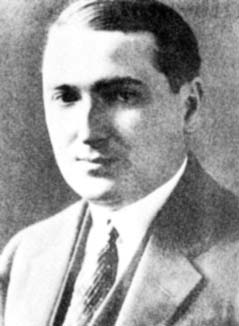
\includegraphics[width=4cm]{figures/EmilLeonPost.jpg}
\end{minipage}
\begin{minipage}{5cm}
\myhref{http://en.wikipedia.org/wiki/Emil_Leon_Post}{Emil Leon Post} \\
\end{minipage}
\end{frame}

\begin{frame}

{\bf Aside:}  To express {\bf PCP} as a language, we let
$L_{\text{PCP}}$ be the language:
$$
\{\langle A,B\rangle|\text{$(A,B)$ instance of PCP with solution}\}
$$

{\bf Example:}  Consider $(A,B)$ given by:

$A=1,10111,10$ \\
$B=111,10,0$

Then $2,1,1,3$ is a solution as:
$$
\underbrace{10111}_{w_2}
\underbrace{1}_{w_1}
\underbrace{1}_{w_1}
\underbrace{10}_{w_3}=
\underbrace{10}_{x_2}
\underbrace{111}_{x_1}
\underbrace{111}_{x_1}
\underbrace{0}_{x_3}
$$
Note that $2,1,1,3,2,1,1,3$ is another solution.  

On the other hand, you can check that:
$A=10,011,101$ \&\
$B=101,11,011$
Does not have a solution.
\end{frame}

\begin{frame}
The {\bf MPCP} has an additional requirement that the first pair in
the solution must be the first pair of $(A,B)$.

So $i_1,i_2,\ldots,i_m$, $m\ge 0$, is a solution to the $(A,B)$
instance of {\bf MPCP} if:
$$
w_1w_{i_1}w_{i_2}\ldots w_{i_m}=x_1x_{i_1}x_{i_2}\ldots x_{i_m}
$$

We say that $i_1,i_2,\ldots,i_r$ is a \df{partial solution} of PCP if
one of the following is the prefix of the other:
$$
w_{i_1}w_{i_2}\ldots w_{i_r}\qquad x_{i_1}x_{i_2}\ldots x_{i_r}
$$
Same def holds for MPCP, but $w_1,x_1$ must be at the beginning.
\end{frame}

\begin{frame}
We now show:

\begin{enumerate}
\item  If {\bf PCP} is decidable, then so is {\bf MPCP}.
\item  If {\bf MPCP} is decidable, then so is $\ATM$.
\item  Since $\ATM$ is {\em not} decidable, neither is {\bf (M)PCP}.
\end{enumerate}
\end{frame}

\begin{frame}
\begin{center}
\fbox{{\bf PCP} decidable $\Longrightarrow$ {\bf MPCP} decidable}
\end{center}

We show that given an instance $(A,B)$ of MPCP, we
can construct an instance $(A',B')$ of PCP such that:
\begin{center}
$(A,B)$ has solution $\iff$ $(A',B')$ has solution
\end{center}

Let $(A,B)$ be an instance of MPCP over the alphabet $\Sigma$.  Then
$(A',B')$ is an instance of PCP over the alphabet
$\Sigma'=\Sigma\cup\{*,\$\}$.

If $A=w_1,w_2,w_3,\ldots,w_k$, then 
$A'=*\textbf{w}_1*,\textbf{w}_1*,\textbf{w}_2*,\textbf{w}_3*,
\ldots,\textbf{w}_k*,\$$.

If $B=x_1,x_2,x_3,\ldots,x_k$, then
$B'=*\textbf{x}_1,*\textbf{x}_1,*\textbf{x}_2,*\textbf{x}_3,
\ldots,*\textbf{x}_k,*\$$.

where if $x=a_1a_2a_3\ldots a_n\in\Sigma^*$, then
$\textbf{x}=a_1*a_2*a_3*\ldots*a_n$.
\end{frame}

\begin{frame}

{\bf For example:} If $(A,B)$ is an instance if MPCP given as:

$A=1,10111,10$ \\
$B=111,10,0$

Then $(A',B')$ is an instance of PCP given as follows:

$A'=*1*,1*,1*0*1*1*1*,1*0*,\$$ \\
$B'=*1*1*1,*1*1*1,*1*0,*0,*\$$
\end{frame}

\begin{frame}
\begin{center}
\fbox{{\bf MPCP} decidable $\Longrightarrow$ $\ATM$ decidable}
\end{center}

Given a pair $(M,w)$ we construct an instance $(A,B)$ of MPCP such
that: 

TM $M$ accepts $w$ $\iff$ $(A,B)$ has a solution.

{\bf Idea:}  The MPCP instance $(A,B)$ simulates, in its partial
solutions, the computation of $M$ on $w$.

That is, partial solutions will be of the form:
$$
\hsh\alpha_1\hsh\alpha_2\hsh\alpha_3\hsh\ldots
$$
where $\alpha_1$ is the initial config of $M$ on $w$, and for all $i$,
$\alpha_i\ra\alpha_{i+1}$.

The string from the $B$ list will always be one config ahead of the $A$
list; the $A$ list will be allowed to ``catch-up'' only when $M$
accepts $w$.
\end{frame}

\begin{frame}
To simplify things,
we may assume that our TM $M$:
\begin{enumerate}
\item  Never prints a blank.
\item  Never moves left from its initial head position.
\end{enumerate}

The configs of $M$ will always be of the form $\alpha q\beta$, where
$\alpha,\beta$ are non-blank tape symbols and $q$ is a state.
\end{frame}

\begin{frame}
Let $M$ be a TM and $w\in\Sigma^*$.  We
construct an instance $(A,B)$ of MPCP as follows:
\begin{enumerate}
\item 
$A$: \hsh  \\
$B$: $\hsh q_0w\hsh$ 

\item 
$A$: $X_1,X_2,\ldots,X_n,\hsh$ \\
$B$: $X_1,X_2,\ldots,X_n,\hsh$ \\
where the $X_i$ are all the tape symbols.

\item To simulate a move of $M$, for all non-accepting $q\in Q$:
\begin{center}
\begin{tabular}{lll}
list $A$ & list $B$ & \\
$qX$     & $Yp$     & if $\delta(q,X)=(p,Y,\rightarrow)$ \\
$ZqX$    & $pZY$    & if $\delta(q,X)=(p,Y,\leftarrow)$ \\
$q\hsh$    & $Yp\hsh$   & if $\delta(q,B)=(p,Y,\rightarrow)$ \\
$Zq\hsh$   & $pZY\hsh$  & if $\delta(q,B)=(p,Y,\leftarrow)$
\end{tabular}
\end{center}
\end{enumerate}
\end{frame}

\begin{frame}
\begin{enumerate}
\setcounter{enumi}{3}
\item If the config at the end of $B$ has an accepting state, then we need
to allow $A$ to catch up with $B$.  So we need for all accepting
states $q$, and all symbols $X,Y$:
\begin{center}
\begin{tabular}{ll}
list $A$ & list $B$ \\
$XqY$    & $q$ \\
$Xq$     & $q$ \\
$qY$     & $q$
\end{tabular}
\end{center}
\item Finally, after using 4 and 3 above, we end up with $x\hsh$ and
$x\hsh q\hsh$, where $x$ is a long string.  Thus we need $q\hsh\hsh$ in $A$ and
$\hsh$ in $B$ to complete the catching up.
\end{enumerate}
\end{frame}

\begin{frame}

{\footnotesize Ex.
%$M=(\{q_1,q_2,q_3\},\{0,1\},\{0,1,B\},\delta,q_1,B,\{q_3\})$,
%\begin{tabular}{c|c|c|c}
%      & 0                     & 1                    & B \\\hline
%$q_1$ & $(q_2,1,\rightarrow)$ & $(q_2,0,\leftarrow)$ & $(q_2,1,\leftarrow)$\\
%\hline
%$q_2$ & $(q_3,0,\leftarrow)$ & $(q_1,0,\rightarrow)$ & $(q_2,0,\rightarrow)$\\
%\hline
%$q_3$ & --- & --- & --- \\
%\end{tabular}
$\delta(q_1,0)=(q_2,1,\rightarrow),
\delta(q_1,1)=(q_2,0,\leftarrow),
\delta(q_1,B)=(q_2,1,\leftarrow)$
$\delta(q_2,0)=(q_3,0,\leftarrow),
\delta(q_2,1)=(q_1,0,\rightarrow),
\delta(q_2,B)=(q_2,0,\rightarrow)$

\begin{tabular}{|l|l|l|l|}\hline
Rule & list $A$ & list $B$      & Source \\\hline\hline
1    & $\hsh$     & ${\hsh}q_101{\hsh}$   &        \\\hline
2    & $0$      & $0$           &        \\
     & $1$      & $1$           &        \\
     & ${\hsh}$     & ${\hsh}$          &        \\\hline
3    & $q_10$   & $1q_2$        & $\delta(q_1,0)=(q_2,1,\rightarrow)$ \\
     & $0q_11$  & $q_200$       & $\delta(q_1,1)=(q_2,0,\leftarrow)$ \\
     & $1q_11$  & $q_210$       & $\delta(q_1,1)=(q_2,0,\leftarrow)$\\ 
     & $0q_1${\hsh} & $q_201${\hsh}     & $\delta(q_1,B)=(q_2,1,\leftarrow)$\\
     & $1q_1${\hsh} & $q_211${\hsh}     & $\delta(q_1,B)=(q_2,1,\leftarrow)$\\
     & $0q_20$  & $q_300${\hsh}     & $\delta(q_2,0)=(q_3,0,\leftarrow)$\\
     & $1q_20$  & $q_310${\hsh}     & $\delta(q_2,0)=(q_3,0,\leftarrow)$\\
     & $q_21$   & $0q_1$        & $\delta(q_2,1)=(q_1,0,\rightarrow)$\\
     & $q_2${\hsh}  & $0q_2${\hsh}      & $\delta(q_2,B)=(q_2,0,\rightarrow)$\\\hline
\end{tabular}
\begin{tabular}{|l|l|l|l|}\hline
4    & $0q_30$  & $q_3$         & \\
     & $0q_31$  & $q_3$         & \\
     & $1q_30$  & $q_3$         & \\
     & $1q_31$  & $q_3$         & \\
     & $0q_3$   & $q_3$		& \\
     & $1q_3$   & $q_3$		& \\
     & $q_30$   & $q_3$		& \\
     & $q_31$   & $q_3$		& \\\hline
5    & $q_3{\hsh}{\hsh}$& ${\hsh}$          & \\\hline
\end{tabular}}
\end{frame}

\begin{frame}
The TM $M$ accepts the input $01$ by the sequence of moves:
$$
q_101\ra
1q_21\ra
10q_1\ra
1q_201\ra
q_3101
$$

We examine the sequence of partial solutions that mimics this
computation of $M$ and eventually leads to a solution.  

We must start with the first pair (MPCP):

$A$: {\hsh} \\
$B$: {\hsh}$q_101${\hsh}

The only way to extend this partial solution is with the corresponding
pair $(q_10,1q_2)$, so we obtain:

$A$: {\hsh}$q_10$ \\
$B$: {\hsh}$q_101{\hsh}1q_2$ 
\end{frame}

\begin{frame}

{\footnotesize
Now using copying pairs we obtain:

$A$: {\hsh}$q_101{\hsh}1$ \\
$B$: {\hsh}$q_101{\hsh}1q_21{\hsh}1$ 

Next corresponding pair is $(q_21,0q_1)$:

$A$: {\hsh}$q_101{\hsh}1q_21$ \\
$B$: {\hsh}$q_101{\hsh}1q_21{\hsh}10q_1$ 

Now careful!  We only copy the next two symbols to obtain:

$A$: {\hsh}$q_101{\hsh}1q_21{\hsh}1$ \\
$B$: {\hsh}$q_101{\hsh}1q_21{\hsh}10q_1{\hsh}1$ 

because we need the $0q_1$ as the head now moves left, and use the
next appropriate corresponding pair which is $(0q_1{\hsh},q_201{\hsh})$ and
obtain:

$A$: {\hsh}$q_101{\hsh}1q_21{\hsh}10q_1{\hsh}$ \\
$B$: {\hsh}$q_101{\hsh}1q_21{\hsh}10q_1{\hsh}1q_201{\hsh}$ 
}
\end{frame}

\begin{frame}

{\footnotesize
We can now use another corresponding pair $(1q_20,q_310)$ right away
to obtain:

$A$: {\hsh}$q_101{\hsh}1q_21{\hsh}10q_1{\hsh}1q_20$ \\
$B$: {\hsh}$q_101{\hsh}1q_21{\hsh}10q_1{\hsh}1q_201{\hsh}q_310$ 

and note that we have an accepting state!  We use two copying pairs to
get:

$A$: {\hsh}$q_101{\hsh}1q_21{\hsh}10q_1{\hsh}1q_201{\hsh}$ \\
$B$: {\hsh}$q_101{\hsh}1q_21{\hsh}10q_1{\hsh}1q_201{\hsh}q_3101{\hsh}$ 

and we can now start using the rules in 4.\ to make $A$ catch up with
$B$:

$A$: $\ldots{\hsh}q_31$ \\
$B$: $\ldots{\hsh}q_3101{\hsh}q_3$ 

and we copy three symbols:

$A$: $\ldots{\hsh}q_3101{\hsh}$ \\
$B$: $\ldots{\hsh}q_3101{\hsh}q_301{\hsh}$ 
}
\end{frame}

\begin{frame}
And again catch up a little:

$A$: $\ldots{\hsh}q_3101{\hsh}q_30$ \\
$B$: $\ldots{\hsh}q_3101{\hsh}q_301{\hsh}q_3$ 

Copy two symbols:

$A$: $\ldots{\hsh}q_3101{\hsh}q_301{\hsh}$ \\
$B$: $\ldots{\hsh}q_3101{\hsh}q_301{\hsh}q_31{\hsh}$ 

and catch up:

$A$: $\ldots{\hsh}q_3101{\hsh}q_301{\hsh}q_31$ \\
$B$: $\ldots{\hsh}q_3101{\hsh}q_301{\hsh}q_31{\hsh}q_3$ 

and copy:

$A$: $\ldots{\hsh}q_3101{\hsh}q_301{\hsh}q_31{\hsh}$ \\
$B$: $\ldots{\hsh}q_3101{\hsh}q_301{\hsh}q_31{\hsh}q_3{\hsh}$ 
\end{frame}

\begin{frame}
And now end it all with the corresponding pair $(q_3{\hsh}{\hsh},{\hsh})$ given by
rule 5.\ to get matching strings:

$A$: $\ldots{\hsh}q_3101{\hsh}q_301{\hsh}q_31{\hsh}q_3{\hsh}{\hsh}$ \\
$B$: $\ldots{\hsh}q_3101{\hsh}q_301{\hsh}q_31{\hsh}q_3{\hsh}{\hsh}$ 

{\bf THEREFORE:} we reduced $\ATM$ to the MPCP.  Now, we can solve
$\ATM$ by producing a carefully crafted instance of MPCP $(A,B)$, and
asking if it has a solution.  If yes, then we know that $M$ accepts
$w$.

Since we have already shown that $\ATM$ is undecidable, MPCP must also
be undecidable.  Thus, PCP is undecidable.

{\bf NEXT:} We can now use the fact that PCP is undecidable to show
that a number of questions about CFLs are undecidable.
\end{frame}

\begin{frame}
Let $A=w_1,w_2,\ldots,w_k$, let $G_A$ be the related CFG given by:
$$
A\longrightarrow w_1Aa_1|w_2Aa_2|\cdots|w_kAa_k|w_1a_1|w_2a_2|\cdots|w_ka_k
$$
Let $L_A=L(G_A)$, the language of the list $A$, and
$a_1,a_2,\ldots,a_k$ are distinct index symbols not in alphabet of
$A$.

The terminal strings of $G_A$ are of the form:
$$
w_{i_1}w_{i_2}\ldots w_{i_m}a_{i_m}\ldots a_{i_2}a_{i_1}
$$

Let $G_{AB}$ be a CFG consisting of $G_A,G_B$, with $S\longrightarrow
A|B$.

$\therefore$ $G_{AB}$ is ambiguous $\iff$ the PCP $(A,B)$ has a
solution.

{\bf Theorem:}  It is undecidable whether a CFG is ambiguous.
\end{frame}

\begin{frame}
$\overline{L_A}$ is also a CFL; we show this by giving a PDA $P$.

$\Gamma_P=\Sigma_A\cup\{a_1,a_2,\ldots,a_k\}$.

As long as $P$ sees a symbol in $\Sigma_A$ it stores it on the stack.

As soon as $P$ sees $a_i$, it pops the stack to see if top of string
is $w_i^R$.  (i) if not, then accept no matter what comes next.  (ii)
if yes, there are two subcases:

(iia) if stack is not yet empty, continue.

(iib) if stack is empty, and the input is finished, reject.

If after an $a_i$, $P$ sees a symbol in $\Sigma_A$, it accepts.
\end{frame}

\begin{frame}

{\bf Theorem:} $G_1,G_2$ are CFGs, and $R$ is a reg.\ exp., then the
following are undecidable problems:
\begin{enumerate}
\item  $L(G_1)\cap L(G_2)\stackrel{?}{=}\emptyset$
\item  $L(G_1)\stackrel{?}{=} L(G_2)$
\item  $L(G_1)\stackrel{?}{=} L(R)$
\item  $L(G_1)\stackrel{?}{=} T^*$
\item  $L(G_1)\stackrel{?}{\subseteq} L(G_2)$
\item  $L(R)\stackrel{?}{\subseteq} L(G_2)$
\end{enumerate}
\end{frame}

\begin{frame}
Proofs: 1. Let $L(G_1)=L_A$ and $L(G_2)=L_B$, then $L(G_1)\cap
L(G_2)\neq\emptyset$ iff PCP $(A,B)$ has a solution.

2.  Let $G_1$ be the CFG for $\overline{L_A}\cup\overline{L_B}$ (CFGs
are closed under union).  Let $G_2$ be the CFG for the reg.\ lang.\
$(\Sigma\cup\{a_1,a_2,\ldots,a_k\})^*$.  

Note
$L(G_1)=\overline{L_A}\cup\overline{L_B}=\overline{L_A\cap L_B}=$
everything but solutions to PCP $(A,B)$.

$\therefore$ $L(G_1)=L(G_2)$ iff $(A,B)$ has no solution.

3.  Shown in 2.

4.  Again, shown in 2.

5.  Note that $A=B$ iff $A\subseteq B$ and $B\subseteq A$, so it
follows from 2.

6.  By 3.\ and 5.
\end{frame}

\end{document}
